\documentclass{article}
\usepackage[utf8]{inputenc}
\usepackage[english]{babel}
\usepackage{graphicx}
\usepackage{pdfpages}

\graphicspath{{image/}}

\title{ROBOTICA}
\author{t.steenhoven }
\date{February 2019}

\begin{document}
\begin{titlepage}
\newcommand{\HRule}{\rule{\linewidth}{0.5mm}}
\center

\textsc{\LARGE Honours Programme }\\[1.5cm]

\textsc{\large Inholland University of Applied Science}\\[.5cm]

\HRule \\[0.4cm]
{ \huge \bfseries Personal Profile of Excellence}\\[0.4cm] % Title of your document
\HRule \\[1.5cm]
\Large

\setlength{\parindent}{0em}

\begin{figure}[!h]
	\centering
	
\includegraphics[width=0.7\textwidth]{shield}
\end{figure}

\begin{table}[!h]
	\centering
	\begin{tabular}{l c l}
		Name &:& Timothy van der Steenhoven \\
		Student nr &:& 522397 \\
		E-mail &:& 522397@student.inholland.nl\\
		Study &:& Computer engineering of applied computer science\\
	\end{tabular}
\end{table}
\newpage
\pagestyle{empty}
\begin{center}
 
    {\LARGE Personal Profile of Excellence}
    \\[4cm]
    
    
    {\Large Timothy van der Steenhoven}\\
    {\large Inholland University of Applied Science}
    \\[.5cm]
    Student ID:\\ 522397 
    \\[2cm]
    Coach:\\
    Cees-Jeroen Bes
    \\[2cm]
    Made for:\\
    Me\\
    Honours Programme
    \\[1cm]
    {\large Groet \today}
\end{center}
\end{titlepage}

\newpage

\tableofcontents

\newpage

\section*{What is excellence?}
Excellence for me is woven in my motto. `Usus est magister optimus' roughly translates into `Practice makes perfect' and that has been my way of learning since I went to school for the first time. \\

During the Honours programme I have put in alot of hours in examining my own learning habits and turning bad habits into slightly less bad habits. In short I have learned about the seven habits of Stephen R. Covey, stared fear in the eyes and discovered a well diverse, open-minded community.\\

Each of the different masterclasses and activities will be elaborated on in the next sections. I will be talking about my first impressions, the speakers themselves and how they have given me alot of different insights. \\

\section{Personal leadership with Egbert Bol}
\subsection{I}
Egbert Bol is difficult to describe in one word. So I'll use three: \textbf{full of energy}.\\

In the first masterclass he stated that his first and foremost priority is to transfer knowledge between eachother. It is one of the crucial methods in being a team. Together Everybody Achieves More. \\

Then he starts with the question: ``What is leadership?'' and that gave me a thought. I have never thought about a thing called `leadership', I thought leadership was self explanatory, but Egbert has proven me wrong. A manager does not have to be a leader and a leader does not have to be a manager. Leaders can be found in many different roles in a company and are not limited to managing positions. Egbert Bol states that the most important attribute for a leader is: ``To see the next thing coming.''\\ 

We proceed to receive insight in paradigms, at this moment I have read the book of Stephen R. Covey for about one or two chapters, and understanding paradigms is a powerfull skill. Paradigms are the ways I see things. I have a personal history as a to-be-nurse and the skills I have learned in those years, I still implement in my day to day activities. \\

\textbf{``Dare to dream and have the guts to do it!''} \\
Egbert Bol, 2019.

\subsection{II}
In the second masterclass from Egbert Bol, I gave a presentation about the shield that I have made. The shield consists of four parts and each part represents a part of me. I have put my shield on the front of this profile.\\

The presentation itself was pretty scary. I am stubborn and my parents always blamed my star sign, which is a lion. The key represents the idea, which I firmly believe, that everybody has their own keys and that you are responsible for your own successes and failures. On the top right I have tried to represent travel. I have fallen in love with it and discovering new places together with people I trust and like gives me a happy feeling. \\

The last part is the wall with the cracks in it. This part is special to me. It represents the lessons people learn from experiences (bricks) that are held together by social interaction, parental love and love for your significant other (mortar). During my life I have had some hardships that I had to work through (cracks).\\

Everybody gets some cracks in their wall eventually. I have learned that I can fill them up together with the people I like and love. I can do it alone, but it is easier with more social interaction/love. \\

\subsection{III}
``Value based leadership is the strongest leadership, but it still had slot of pitfalls.''\\
Egbert Bol, 2019\\

In the third masterclass from Egbert Bol, we've talked through the structure of a habit. The three conditions for a habit to exist, is:
\begin{enumerate}
	\item Knowledge, what to do about something  and why.
	\item Skill , knowing how to do something
	\item Desire, wanting to do something.	
	\end{enumerate} 
Together these form a habit. The first three habits of Covey are there to develop leadership of your own life. Be proactive, begin with the end in mind and put first things first. \\

Since a few years I have developed a proactive way of thinking. If a problem arises, e.g. a teacher that has not returned my marks yet. While I complain about it with my fellow students I also send an e-mail to the teacher or speak to him/her about the missing mark. In most of the cases I get a direct answer and the marks are visible the next week. \\

The second habit is harder for me to visualize at this point. Before Honours, I have not given it a thought. Begin with the end in mind. The example from the book of Covey states that the reader should close his/her eyes and try to visualize their 80\textsuperscript{th} birthday.\\

Well, I did the exercise and I visualised my 80\textsuperscript{th} birthday as a party at a restaurant that has a table ready for 40 people. These 40 people consist of my wife, twin brother, sisters, children, my children their children and a couple of friends. \\

It gave me alot of insight for habit number three, put first things first. I have come to the conclusion that health and family are equally important priority's in my life.\\

And that ends the masterclasses from Egbert Bol. I have learned alot of him about leadership, paradigms and that in communication, your energy can have a lot of influence.

\section{Dog Coaching 16-02-19}
Saturday the 16th of February, we have been informed that the dogs will be coaching us and not the other way around. This is something I have not experienced yet and I am excited to do it. \\

We were welcomed on the property with a cozy atmosphere. The house was lovely and I really felt welcomed. After a brief introduction to the instructors, everybody went outside for the first exercise with Brena, see figure 1.\\

\begin{figure}[!h]
	\centering
	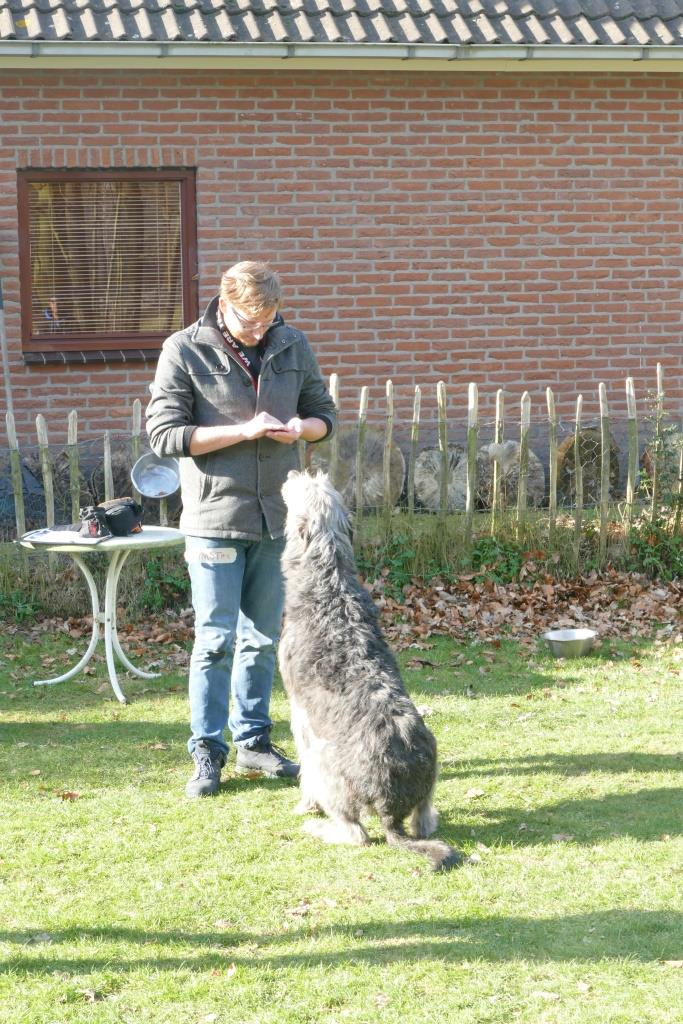
\includegraphics[width=0.4\textwidth]{brena}
	\label{fig:Brena}
	\caption{Brena}
\end{figure}

Brena has learned me to be open about my wishes. I can say to Brena that I want her to sit, but eventually my non-verbal communication plays a big role in this. First I have to picture the something that I want from Brena, in this case I want her to sit. Then I have to adjust my stance to Brena and ask her clearly to sit.\\

This is a good example of the second habit of Covey, begin with the end in mind.\\


After the exercise with Brena we went on with the second exercise with the dog Marley, I have displayed a picture of him in figure \ref{fig:Sebastian}.  

\begin{figure}[!h]
	\centering
	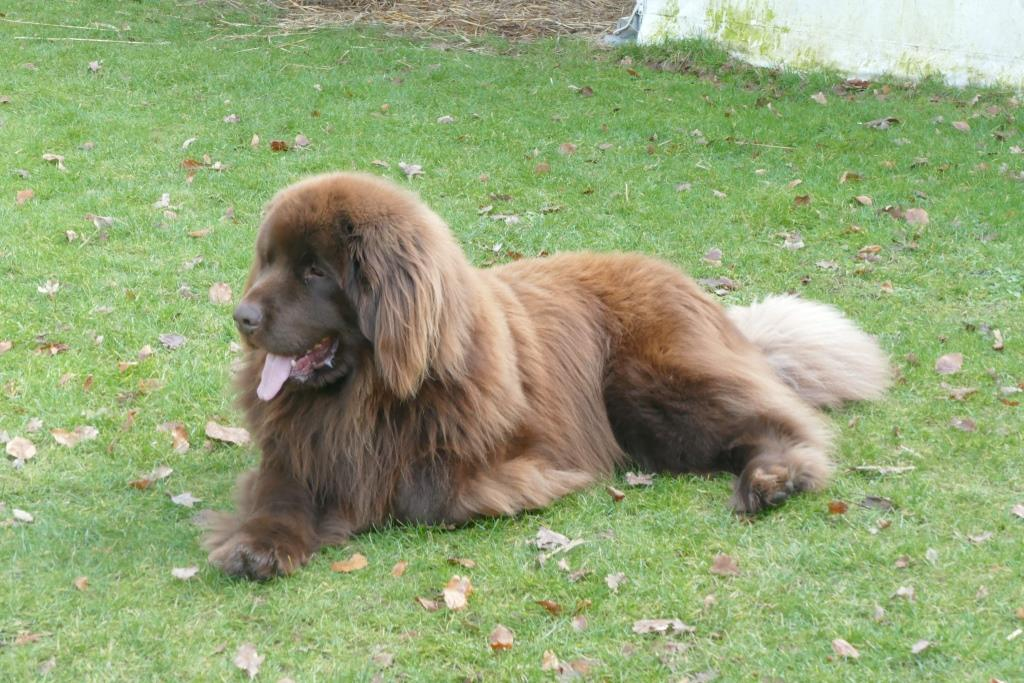
\includegraphics[width=0.6\textwidth]{sebastian}
	\label{fig:Sebastian}
	\caption{Marley}
\end{figure}
When Marley first walked around the corner, we all saw an absolute unit of a dog. Marley is big, young and full of energy. With Marley we learned to invite him to the pack as a pack, instead of asking him directly to do the exercise. \\

After a brief time-out we first interacted with Marley by petting him and showing him that we want him to help our pack. Then we hit a second wall, Marley stopped. He was not motivated to do the exercise with us. Somebody asked the instructor is the Marley is motivated by treats ans he sure was.\\

The following obstacle was coördination. Now everybody knew what we had to do, but everybody was following eachother and there was no clear communication in the pack. Tim came with the idea to create a coördinator role and communicate every step within the pack. This worked like a charm.\\

\begin{figure}[!h]
	\centering
	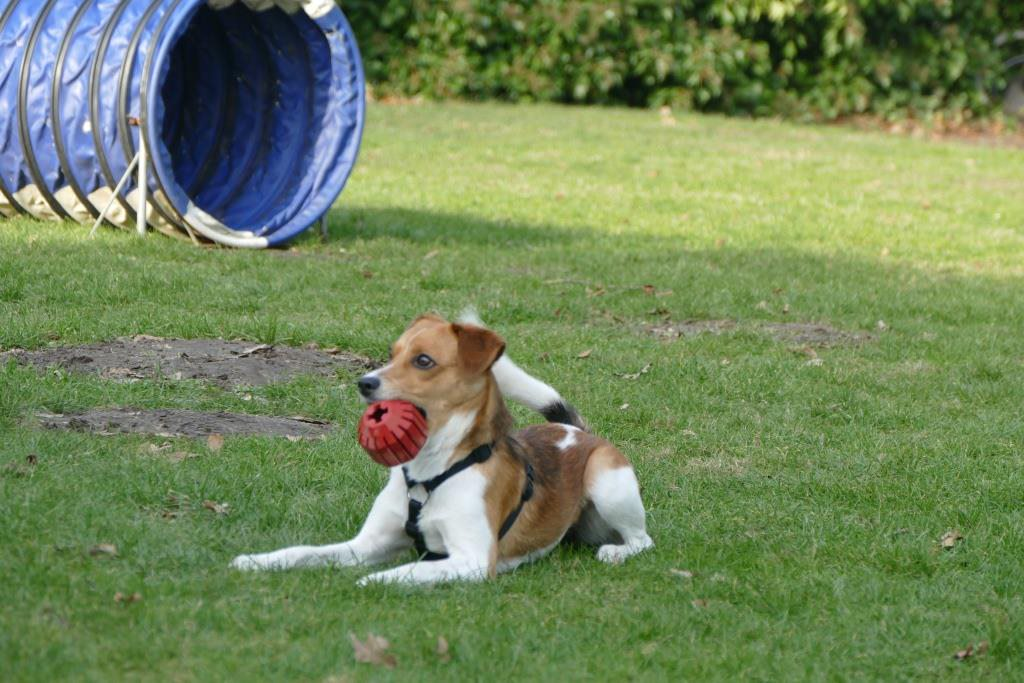
\includegraphics[width=0.6\textwidth]{yuna}
	\label{fig:Yuna}
	\caption{Yuna}
\end{figure}

After a lunch break we went outside for the third exercise with the last dog: Yuna, figure 3. Yuna is the youngest and newest member of the pack and has a lot of energy. During this exercise I was the coordinator. In the beginning I had the idea that I had to plan every step of the exercise, but the instructor quickly told me to ask for input from the pack. \\

This changed a few things in the exercise. Yuna is a young dog and that is the reason that she can not focus for too long on the object/person. Eventually the exercise was about getting Yuna to complete a custom course with every pack member, but in the end we all took care for one part of the course.\\

When everybody was doing their part in completing the course I felt happy. The pack and Yuna completed the course by doing it together. In figure 4 I have added a nice memory of that day.

\begin{figure}[!h]
	\centering
	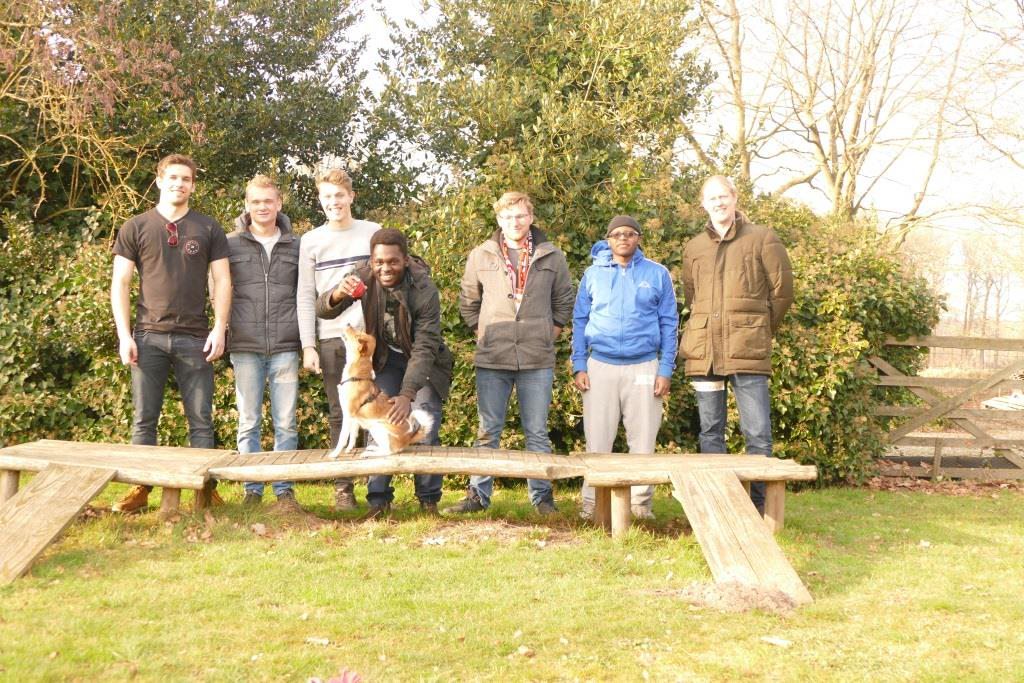
\includegraphics[width=0.7\textwidth]{Dogcoaching}
	\label{fig:Dogcoaching}
	\caption{Group foto at the end of the dog coaching.}
\end{figure}
\newpage
\section{Bootcamp}
First thing I have to say about the bootcamp is that the activities were mentally and physically straining. Going to bed at 3 A.M. and then stand up at 7 A.M. for breakfast is pretty damaging to the body and mind.\\

But let me start at the beginning. I have never done anything like this before and the my senior Honours students did not want to spill any beans about the bootcamp. That only sparked my interest even more.\\

When I arrived, dinner was almost done and the whole community was split into two groups with captains in each team. This is the general setup for every exercise. The first exercise was a `small' walk with the coordinates we have been given. \\

The second day began with exercises in the `backyard' of the house. I have made a picture of it, see figure 5.
\begin{figure}[!h]
	\centering
	\includegraphics[width=0.6\textwidth]{thewall2}
	\label{fig:thewall2}
	\caption{The path to `the wall'. It is roughly 30m high.}
\end{figure}

A lot of exercises were build on the same concept: trust the partner in front of you for the correct instructions and pass them on to the partner in the back. In the first exercise, the team I was in had to walk down an angled flat rock while somebody else secured the rope. In my case my partner was Tim. I have to lean forward for at least 45 degrees to stand up `straight'.\\

At first I was scared, but after a few reassuring thumbs up from Tim I pushed myself to lean forward. After this first step, it was a cakewalk to walk down the rock. This exercise taught me that the first step is scary most of the time, but after taking the first step it all becomes easier.\\

The following photo's are from the wall in comparison to Tim (figure 6) and the view from the top of the wall (figure 7 \& 8).


\begin{figure}[!h]
	\centering
	\includegraphics[width=0.6\textwidth]{thewall}
	\label{fig:wall}
	\caption{The wall in comparison to Tim after abseiling from inside the wall.}
\end{figure}

\begin{figure}[!h]
	\centering
	\includegraphics[width=0.6\textwidth]{view1}
	\label{fig:view1}
	\caption{The view from atop the wall.}
\end{figure}
\begin{figure}[!h]
	\centering
	\includegraphics[width=0.6\textwidth]{view2}
	\label{fig:view2}
	\caption{The view from atop of the wall.}
\end{figure}

The most memorable moment from the bootcamp was the stretcher walk. I assume that the person reading this profile knows about the stretcher walk. Personally it was one of the biggest mental and physical challenges I had in my life. We had to take the two lightest community members on the stretchers for about 20km without turning back. \\

The first few kilometres I was fine, but along the way people started to doubt the meaning of the exercise and were not willing to pour their energy in the exercise. That moment Hans provided us with one of the most motivating speeches I have ever had. He basically told us to suck it up and there is no return. Everybody is in it together and everybody is doing this together. \\

This speech pushed me to carry the stretcher for a few more kilometres, then the next obstacle surfaced. My muscles became sore the more I was carrying the stretcher. Everybody around me had the same problem, some more than others. Along the way it became worse and worse and the last 6 kilometres I must have walked pure on mental power
\newpage
A few people who have inspired me during this trip were:
\begin{itemize}
	\item Tino\\
	Always ready to perform and fit for the army. He tries his best to complete the task he has been given without complaining. It is unbelievable.
	\item Kim\\
	Kim carried the stretcher for a lot of kilometres. I do not know exactly how much but she showed grit. She complained, but we all did. The biggest difference was that she found humor in every situation and pushed us all to step up.
	\item Miguel \& Tim\\
	This duo is insane. These are the only words I have. They carried the stretcher the whole way on their shoulder and tried to find competition in this bootcamp. I walked with them for a few kilometres and every time I thought about stopping for a minute I was pushed mentally to a new limit by these two. 
\end{itemize}  

At the end of the stretcher walk I thought about giving up. I was physically broken and was about to break mentally too. Fred picked up on this and offered advice/help. It was only a few kilometres back to the cabin and I had the feeling that I held back my community. \\

At the end of the stretcher walk, we all went into the cabin to celebrate the completion of the most difficult task we did this bootcamp. I though before the walk that I knew myself pretty well, including my boundaries but I was wrong. I learned that every activity in life may present a unique problem and it will be my flexibility that will help me overcome those problems.

\newpage
\section{Business Skills with Simon Palser}

Simon Palser has been with the Inholland University of Applied Sciences before it was named Inholland. He has been around for a long time and likes to spark discussions within the community. \\ 

My first impression of him was that he was so energetic, it was almost annoying. Behind that energy there was a man that has a lot of experience in the field op communication. \\

He has shown us that engineers are communicating more and more, because of the following activities: 
\begin{itemize}
	\item Engineer need to sell their ideas.
	\item Create clear written content.
	\item Face to face communication, an engineer does not work in the back of a shed anymore these days.
	\item Engineers have to give presentations in front of big groups these days. 
\end{itemize}

With this made clear to us he asked a unexpected question: ``How would you put being a Honours student on your resume?'' I thought by myself: ``I am an Honours student, so I put it as simple as that on my resume.''\\

 Simon then proceeded to ask one student to share his thought. One student answered my thought and Simon responded with: ``Yes, but no. The way you put it, the Honours programme is not special, but you have done alot of things to get in this program. You were \textbf{selected} because you are willing to put in a lot of effort.''\\

``Don't downplay your own achievements!'' Simon said. I am familiar with having little faith in my achievements, because I believe that my achievement is something in the past, but this sentence, spoken by Simon Palser, made me think about my achievements.\\

 Sure, I have a few diploma's, but I also have a home that I rent with my girlfriend, a lot of kind fellow students at Inholland Alkmaar and a nice community at Honours. In my worklife I have climbed the ranks to a managing position in one of the biggest producers of Europe, only to drop it for a new study. The moment I realised this, I found some courage in my achievements.\\
\newpage
\section{Personal Entrepeneurship with Peter de Kock}
This masterclass was given by Peter de Kock, the head of the undercover division of the dutch police. Peter de Kock has had a few interests in his life and it all started with his film making career.

``\textbf{The power of the narrative.}''\\
Peter de Kock, 2019.\\

Peter starts with an impressive story about his life als a film maker and the confrontation with an terrorist that became the student. At that moment I had a weird feeling about Peter that I couldn't place. This man talks positively to us, despite the very dangers he has faced. \\

He then proceedes to tell us about our own stories and that we are responsible for our own narratives. It is ease to say to people the `us and them' part fo a story, but what is in between? Which parties are affected and what are their views of the story?\\

I have not talked about the movies Peter showed us during the masterclass. The movies made me a bog impact on me. One of the movies he showed, was of Britisch journalist John Cantlie. In the movie John explained that IS is not losing ground and that American troops are actually helping IS by supplying them with food and weapons. \\

The movie impacts me a lot, because something feels off in the way John speaks. The context, background and introduction are all positive to his story, but I find it hard to believe he is not held under gun point while doing this. John tells in his movies he is reporting this to tell the world the whole story and not just how the West media represents it to the people.\\

The movies gave me a lot of thought on `news' in the world. Sometimes I see an article stating that a city has been freed by bombing half the city to the ground and think by myself, how is that different than the violence of 70 years ago? And what defines a victory? Please do not misunderstand me, but since the masterclass from Peter de Kock I am feeling more sceptical about `news'.\\

I am trying to first gather more information than to blindly accept the information I have been fed and I feel that this is a powerful progression in my mindset as a student/engineer-to-be.

\newpage
\section{Coaching session 1}
In the first coaching session on the 9\textsuperscript{th} of May 2019 we used the GROW model made by Sir John Whitmore. In table \ref{tab:GROW} you will find the filled in GROW model.

\subsection{GROW model}
\begin{table}[!h]	
	\centering
	\caption{Filled in GROW-model.}
	\label{tab:GROW}
	\begin{tabular}[width=0.8\textwidth]{||p{\textwidth}||}
		\hline
		\textbf{Goal}\\\hline
		\textit{I want to fully trust my fellow students. I am aware that his means that I will be having less control, so I can fulfill my potential within our project.}''\\\hline
		\textbf{Current Reality}\\\hline
		At the moment I am a control freak and my teammates and I can not fulfill our full potential. \\\hline
		\textbf{Explore the Options}\\\hline
		The options I have are:
		\begin{itemize}
			\item Work towards an open dialog.
			\item Set up prerequisites with my team. So everybody has the same mindset.
			\item Develop my interpersonal skills. 
		\end{itemize}\\\hline
		\textbf{Establish the Will}\\\hline
		The way that I am going to work towards my goal is to ask my team for TIPS and TOPS.
		\begin{itemize}
			\item TIPS: Which advise can I take with me to the next project?
			\item TOPS: What did I do well?
		\end{itemize} \\\hline
	\end{tabular}
\end{table}
\newpage

\section{Wheel of Life}
The wheel of life is a tool that helps me to visualize the aspects of life I prioritize. The wheel is attached as appendix \ref{app:wol}

\begin{itemize}
	\item Family\\
	I have given the aspect family a 5 because filling in the wheel made me realise that I do not speak to my family as often as I would like to. To improve that aspect of my life I would like to meet my family more.
	\item Friends\\
	Friends scored high, because at the moment I have a couple of good friends and a bunch of friends from school.
	\item Health\\
	At the moment I'd like to exercise more, but the number I gave it represents how I feel right now. I do not get sick often en I feel well rested after a good night's sleep.
	\item Career\\
	My career is at a standstill at the moment. This year in school pushed me to my mental limits en I have not yet found a way to let loose of my new knowledge. This will be an important next year, when I will be going on an internship.
	\item Love\\
	I am happy with my girlfriend at the moment and our situation right now. She is almost done with her education. After that we want take out relationship to the next step.
	\item Money\\
	I am not a materialist, but as a student money can be tight at the end of the month. I would like to save up enough to buy our first house in the coming 5 years.
	\item Fun\\
	Fun gets a high number from me, because lately I have been having a lot of fun. Discovering new programming languages, getting good grades, going out to party with friends, but I have substraced a few points from the scoren for one reason.\\
	
	I have been neglecting my personal fun. Sometimes I have to do some things I like without somebody else. In order to advance my own `Fun' I have to plan some personal activities. 
\end{itemize}





\section{Coaching session 2}
The last coaching session took place in Delft on 22\textsuperscript{nd} of May 2019, right before the end of the Honours program. In this coaching session we spoke about the Honours programme and what my opinion is of it.\\

I told Cees-Jeroen Bes that everything that was told to me last year, was true. I was told that the Honours programme would be the biggest mental/emotional/physical challenge I have faceda and it was all true.\\

I am still amazed by the masterclasses and the speakers at those masterclasses. They are people who have done what they enjoy and made it marketable. My Cees-Jeroen and I have spoken about the habit that speaks to me the most and I had already thought about it before.\\

The habit I need to work on the most in habit 2: ``Begin with the end in mind.'' As I stated earlier, I have not given the rest of my life some thought. I find it difficult to picture myself over 3 years or 5 years or 10 years. \\

Cees-Jeroen told me that that is normal in life. You do not know what will happen in de near future, but you can steer towards your goals with the activities that you are doing. So the coming year I will be working towards the goal I already stated the section about Egbert Bol his masterclass.\\

  




\newpage
\section{appendix}
\appendix
\subsection{Wheel of Life}\label{app:wol}
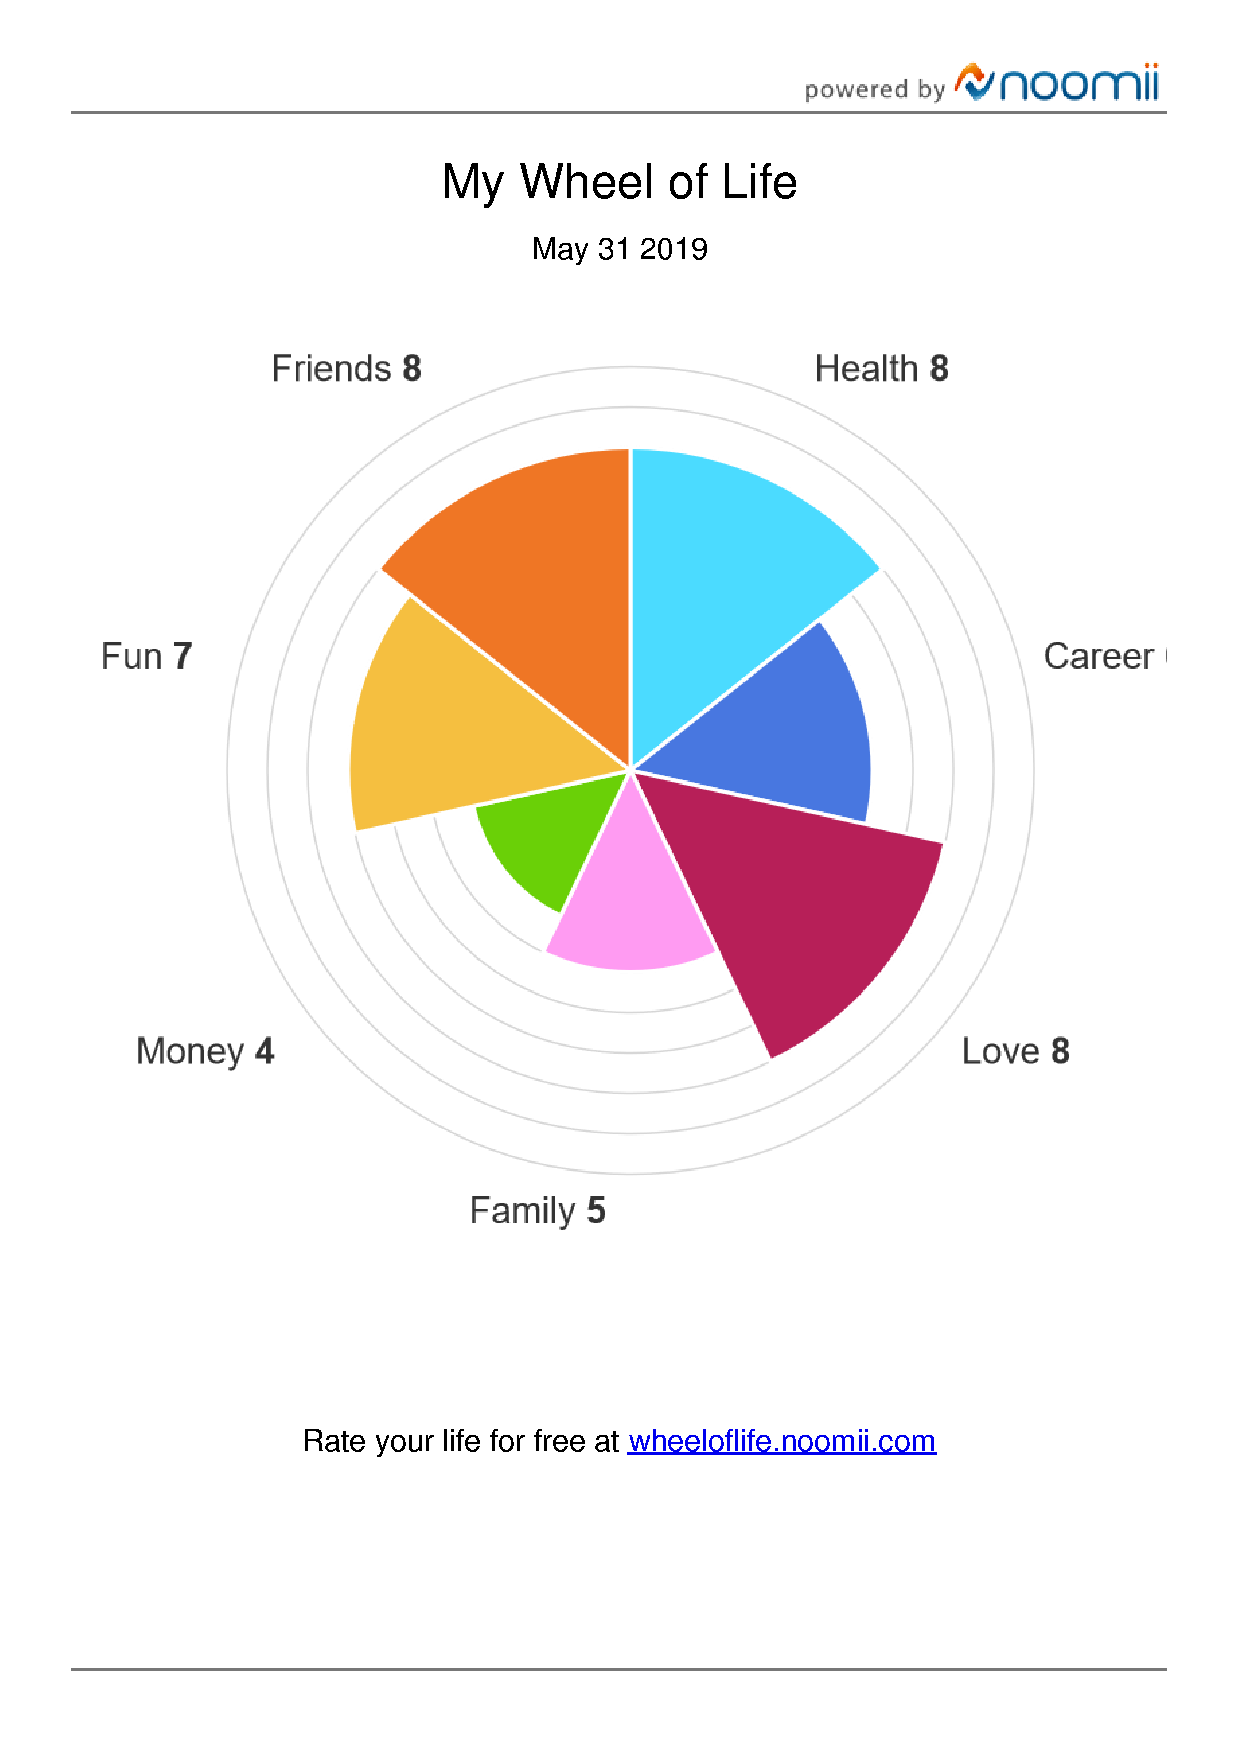
\includepdf[pages={1}]{wol}






\end{document}